\section{Genetics}

\begin{multicols}{2}


\section*{Genetic Materials}


\subsection{Chromatid Models} % VSO 53

\begin{center}
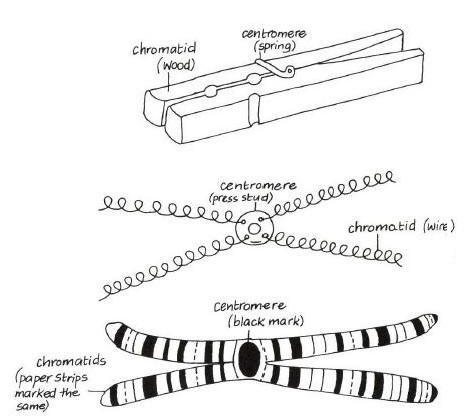
\includegraphics[width=0.49\textwidth]{./img/vso/chromatid.jpg}
\end{center}

\begin{description*}
%\item[Subtopic:]{}
\item[Materials:]{Clothespin, wire, washer/button, paper strips}
%\item[Setup:]{}
\item[Procedure:]{Construct the chromatid models as shown.}
%\item[Hazards:]{}
%\item[Questions:]{}
%\item[Observations:]{}
\item[Theory:]{During the late stage of prophase in mitosis each chromosome can be
seen as 2 parts, called chromatids. These chromatids are joined
together by the centromere.}
%\item[Applications:]{}
%\item[Notes:]{}
\end{description*}

\subsection{DNA Zipper} % VSO 52

\begin{center}
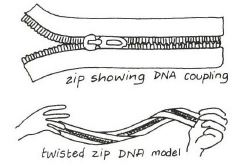
\includegraphics[width=0.4\textwidth]{./img/vso/dna-zipper.jpg}
\end{center}

\begin{description*}
%\item[Subtopic:]{}
\item[Materials:]{Zipper}
%\item[Setup:]{}
%\item[Procedure:]{}
%\item[Hazards:]{}
%\item[Questions:]{}
%\item[Observations:]{}
\item[Theory:]{DNA is wound in a double helix.
The strands of the helix are chains
of sugars and phosphates. The 2
strands of the helix are linked
together by bridges made of pairs
of organic nitrogenous bases
which are joined to the sugar
molecules. A zip provides a good
visual analogy.}
%\item[Applications:]{}
%\item[Notes:]{}
\end{description*}

\columnbreak

\subsection{DNA Helix Model}

\begin{center}
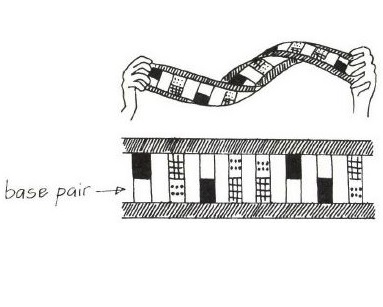
\includegraphics[width=0.45\textwidth]{./img/vso/dna-helix.jpg}
\end{center}

\begin{description*}
%\item[Subtopic:]{}
\item[Materials:]{Card/paper strips, 4 colours}
%\item[Setup:]{}
\item[Procedure:]{Make your helix model
from strips of strong card or
paper. It should be strong enough
to twist as shown.}
%\item[Hazards:]{}
%\item[Questions:]{}
%\item[Observations:]{}
\item[Theory:]{A gene can have a sequence of up
to 1000 base pairs in a DNA
molecule. }
%\item[Applications:]{}
%\item[Notes:]{}
\end{description*}

\subsection{DNA Extraction} % Shika 230 PIC!!!

%\begin{center}
%\includegraphics[width=0.4\textwidth]{./img/.jpg}
%\end{center}

\begin{description*}
%\item[Subtopic:]{}
\item[Materials:]{Salt, soap, water, methylated spirit, bottle}
%\item[Setup:]{}
\item[Procedure:]{Prepare a salt solution by mixing with water. Have students swish the solution in their mouths for about a minute and then spit into a container. Add this to a soap solution and gently swirl for a few minutes. Pour methylated spirit down the inside of the container to form a layer on top.}
%\item[Hazards:]{}
%\item[Questions:]{}
\item[Observations:]{Transparent strands of DNA should precipitate at the boundary between the two layers. Strands can be picked up with a toothpick.}
\item[Theory:]{The enzymes in the soap break down the lipids of the nuclear membranes, releasing the DNA. Salt neutralizes the DNA by providing `+' ions. The DNA slowly rises to the alcohol layer above the water.}
%\item[Applications:]{}
%\item[Notes:]{}
\end{description*}

\columnbreak

\subsection{DNA Model Game} % VSO 52

\begin{center}
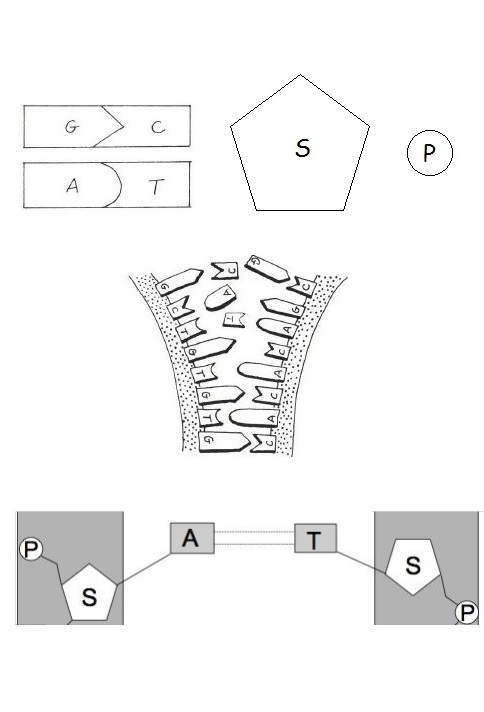
\includegraphics[width=0.45\textwidth]{./img/dna-game.jpg}
\end{center}

\begin{description*}
%\item[Subtopic:]{}
\item[Materials:]{Card/paper, scissors}
\item[Setup:]{Cut out pieces of card to
represent the paired bases, sugars and phosphate groups.}
\item[Procedure:]{Construct a DNA model by correctly joining the parts of the nucleotide. The phosphate group (P) should be atop the deoxyribose sugar (S) and the
base pairs should bond to the deoxyribose sugar as shown. Students must match the bases to
`zip up' the DNA molecule.}
%\item[Hazards:]{}
%\item[Questions:]{}
\item[Observations:]{The bases
always combine in the same pairs:
thymine with adenine and
cytosine with guanine.}
\item[Theory:]{DNA is a double-stranded helical (spiral) molecular chain that is found in the nucleus of the cell. It contains the genetic information of organisms. DNA is made up of many \emph{nucleotides}. The components of a DNA nucleotide are a deoxyribose sugar, phosphoric acid, and an organic base. The four bases of DNA are guanine, cytosine, adenine, and thymine. In humans, DNA determines physical features such as the colour of the skin, eyes, and hair as well as a person's height and the presence or absence of genetic disorders.}
%\item[Applications:]{}
%\item[Notes:]{}
\end{description*}

\columnbreak

%==================================================================================================%

\section*{Inheritance}


\subsection{Mendelian Inheritance} % Shika 231 PIC!!!

%\begin{center}
%\includegraphics[width=0.4\textwidth]{./img/.jpg}
%\end{center}

\begin{description*}
%\item[Subtopic:]{}
\item[Materials:]{Many beans and maize seeds}
%\item[Setup:]{}
\item[Procedure:]{Provide many of each seed to each student or group. Beans represent a dominant allele (Z) and maize seeds represent a recessive allele (z). Have students cross two heterozygotes (e.g. Zz $\times$ Zz) by making a mixture of Zz (50\% beans and 50\% maize) for both the mother and father. To make an offspring, take one seed from each pile. Repeat at least 20 times and record each offspring and its genotype.}
%\item[Hazards:]{}
%\item[Questions:]{}
\item[Observations:]{Several combinations are possible: ZZ, Zz, zZ and zz}
\item[Theory:]{In sexual reproduction, each parent gives the offspring one copy of each gene. If the offspring has even one dominant allele (ZZ, Zz or zZ), it will show the dominant trait Z. A combination of zz reveals the recessive trait.}
\item[Applications:]{Repeat the activity for different heterozygotes (e.g. ZZ $\times$ zz, Zz $\times$ zz, etc.). Have students calculate the probability of an offspring carrying each combination and exhibiting each genotype.}
%\item[Notes:]{}
\end{description*}

%==================================================================================================%

\section*{Sex Determination}


\subsection{Determining Sex of a Child}

\begin{center}
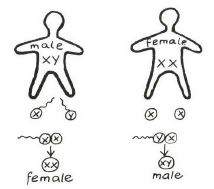
\includegraphics[width=0.4\textwidth]{./img/vso/sex-determination.jpg}
\end{center}

\begin{description*}
%\item[Subtopic:]{}
\item[Materials:]{Card/paper}
%\item[Setup:]{}
\item[Procedure:]{Cut out 2 shapes, one to
represent a male (labeled XY), the
other a female (labeled XX). Cut
out 4 small circles. Label 3 of
them X and label the other Y.
These shapes represent the
gametes. Move sperm and eggs
together to represent fertilisation
and sex determination.}
%\item[Hazards:]{}
%\item[Questions:]{}
%\item[Observations:]{}
\item[Theory:]{An offspring having 2 X gametes will be a female, while a Y gamete results in a male.}
%\item[Applications:]{}
%\item[Notes:]{}
\end{description*}

%==================================================================================================%

%\section*{Variation}
%
%
%\subsection{Mutation Models} % [New - PIC!!!] Bio F4 77
%
%%\begin{center}
%%\includegraphics[width=0.4\textwidth]{./img/.jpg}
%%\end{center}
%
%\begin{description*}
%%\item[Subtopic:]{}
%\item[Materials:]{}
%\item[Setup:]{}
%\item[Procedure:]{}
%\item[Hazards:]{}
%\item[Questions:]{}
%\item[Observations:]{}
%\item[Theory:]{}
%\item[Applications:]{}
%\item[Notes:]{}
%\end{description*}

%==================================================================================================%


\end{multicols}

\pagebreak